\section[Comparision]{Comparision}


\begin{figure} \centering
  {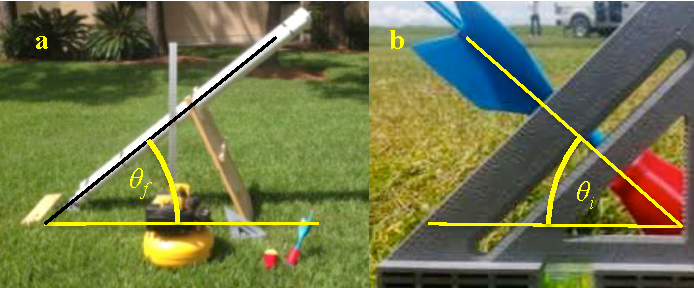
\includegraphics[width=\columnwidth]{ral2016/CannonPicture}}
 \caption{A pneumatic launcher for SeismicDarts.  Ballistic dart deployment has limited usefulness because the incident angle is equal to the firing angle.} 
 \label{fig:CannonPicture}
\end{figure}

\begin{figure*}[htb]
\centering 
\vspace{1em}
%\renewcommand{\figwid}{0.48\columnwidth}
\begin{overpic}[width =\figwid]{ral2016/sim1_1.pdf}
\end{overpic}
\begin{overpic}[width =\figwid]{ral2016/sim1_2.pdf}
\end{overpic}
\begin{overpic}[width =\figwid]{ral2016/sim1_3.pdf}
\end{overpic}
\begin{overpic}[width =\figwid]{ral2016/sim1_4.pdf}
\end{overpic}
\caption{Screenshots of simulations that were performed to estimate time take by different sensors surveying 100x100 m grid: a.) only SeismicSpiders b.) SeismicDarts and deployment system c.) heterogeneous system d.) human workers.
\label{fig:Sim_overview}}
\end{figure*}

\subsection{Ballistic Deployment}
To compare an alternative deployment mechanism we built the pneumatic cannon shown in Fig.~\ref{fig:CannonPicture}a.
The pneumatic cannon is U-shaped,  2 m in length, with a 0.1 m (4 inch) diameter pressure chamber and a 0.08 m (3 inch) diameter firing barrel, connected by an electronic valve (Rain Bird JTV/ASF 100). 
The cannon is aimed by selecting an appropriate firing angle $\theta_f$, azimuth angle, and chamber pressure.  
The reachable workspace is an annular ring whose radius $r$ is a function of the firing angle and initial velocity $v$. 
Neglecting air resistance, this range is found by integration:
\begin{align}
r = \frac{v^2}{g} \sin( 2 \theta_f )
\end{align} 
Initial velocity is limited by the maximum pressure and size of the pressure chamber.
The cannon used  SCH 40 PVC, which is limited to a maximum pressure of 3 Mpa (450 psi).

We charged our system to 1 Mpa (150 psi), and achieved a range of $\approx$ 150 m.
This range is considerably smaller than the UAV's range, which when loaded can complete a round trip of $\approx 1.5$ km.

A larger problem, illustrated in Fig.~\ref{fig:CannonPicture}, is that angle of incidence $\theta_i$ is equal to the firing angle $\theta_f$. 
Maximum range is achieved with $\theta_f = 45^\circ$, but this angle of incidence reduces the geophone sensitivity to $\cos(\theta_f )\approx 0.7$.
The placement accuracy of the cannon is lower than the UAV because a fired dart must fly over a longer distance than a dropped dart. 
Safety reasons also limit applications for a pneumatic launcher.





\begin{table} \centering
  {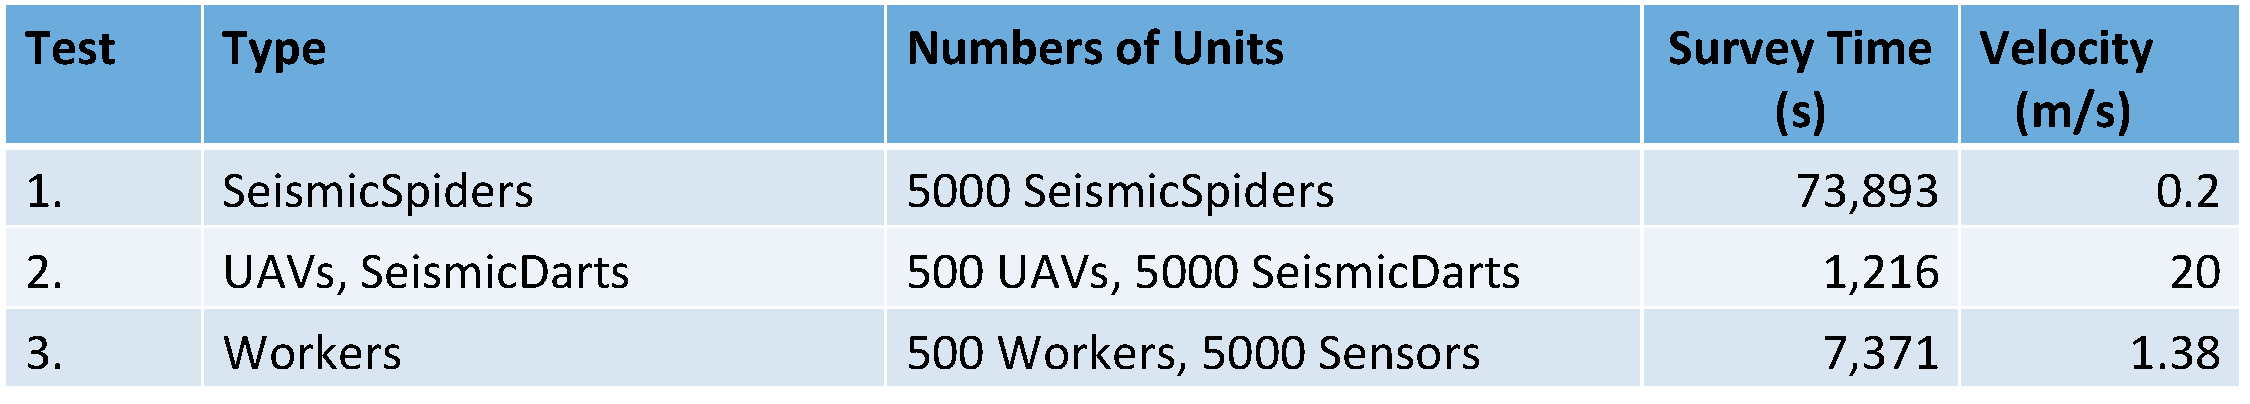
\includegraphics[width=\columnwidth]{ral2016/simulation_table.pdf}}
 \caption{Comparison of different  deployment modes highlights the efficiency of UAV deployment.} 
 \label{tab:Sim_table}
\end{table}

\begin{figure} \centering
  {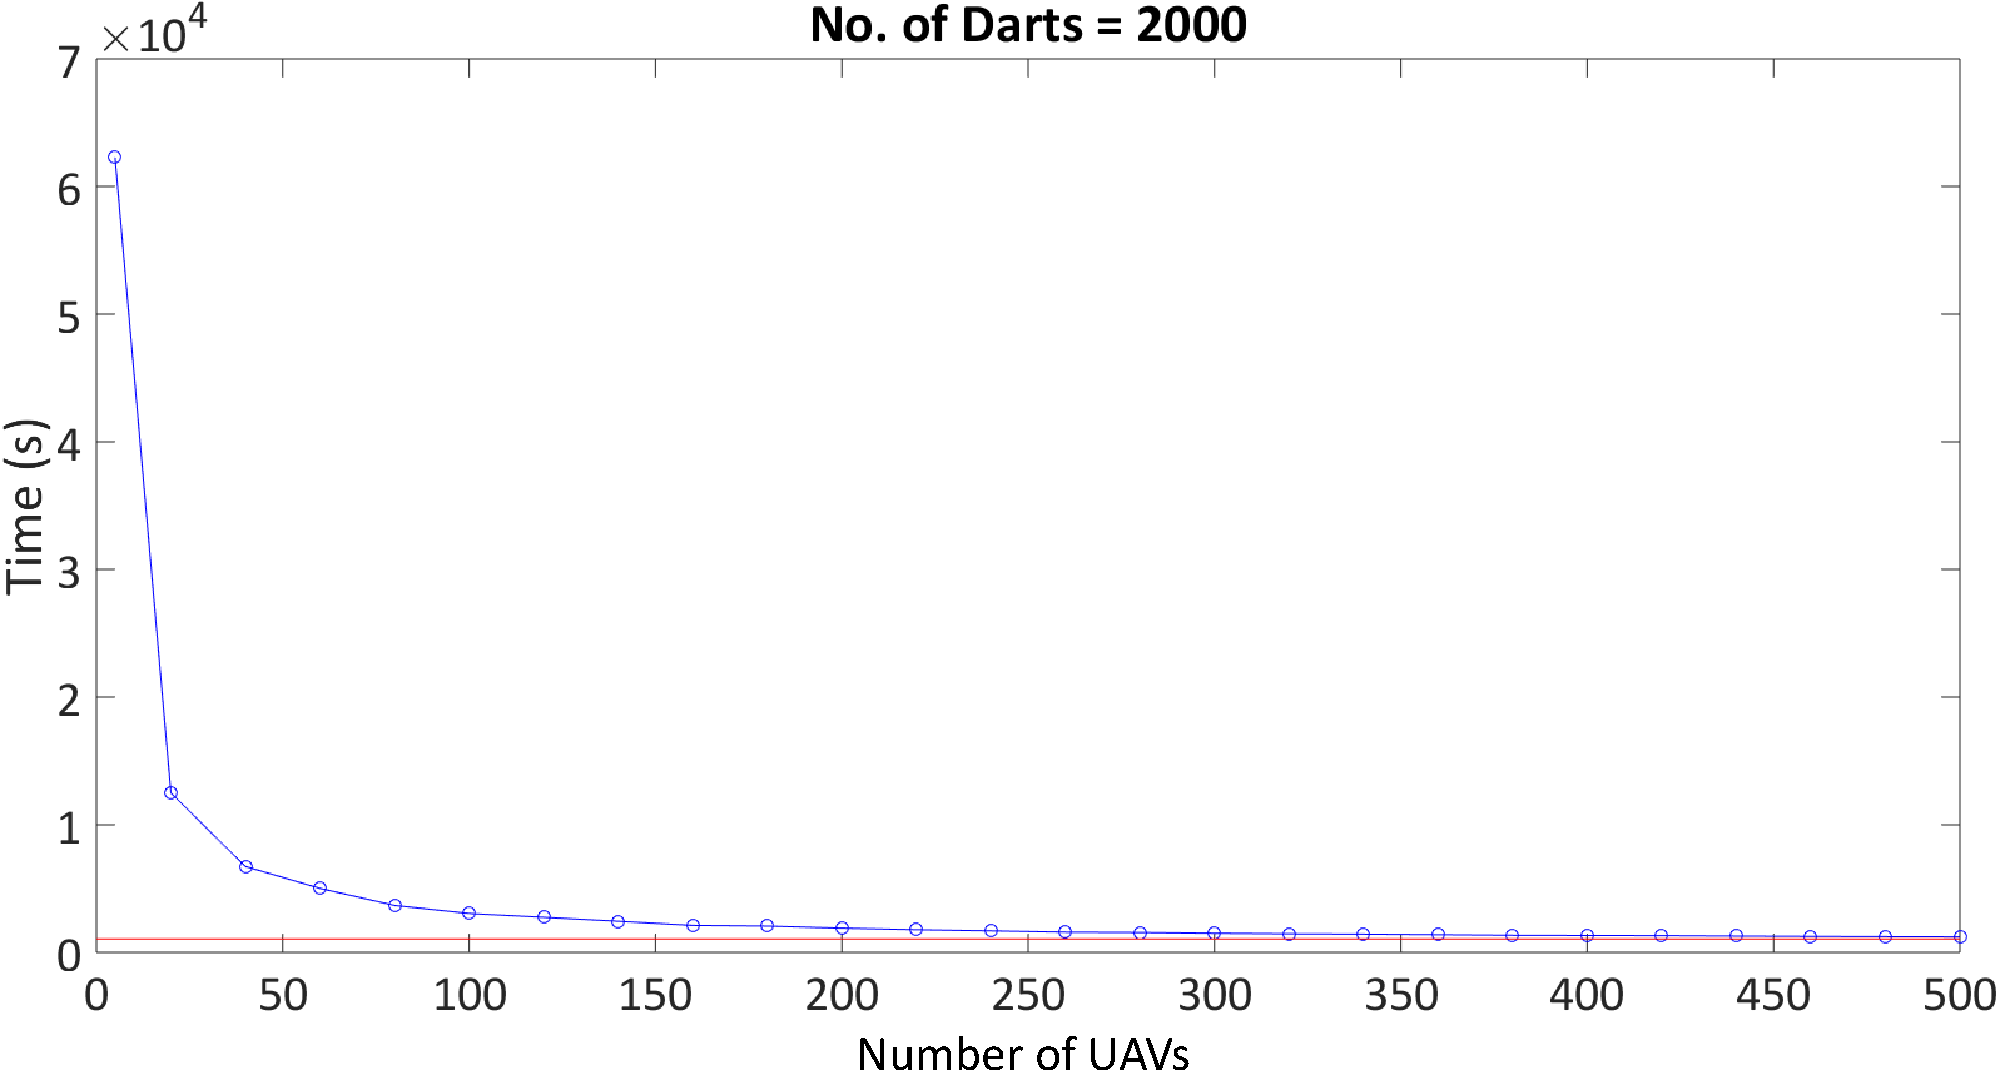
\includegraphics[width=\columnwidth]{ral2016/DronevsTime.pdf}}
 \caption{Survey time for a 1km x 10 km region for different numbers of UAVs.} 
 \label{fig:DronevsTime}
 \vspace{-1em}
\end{figure}

\begin{figure} \centering
  {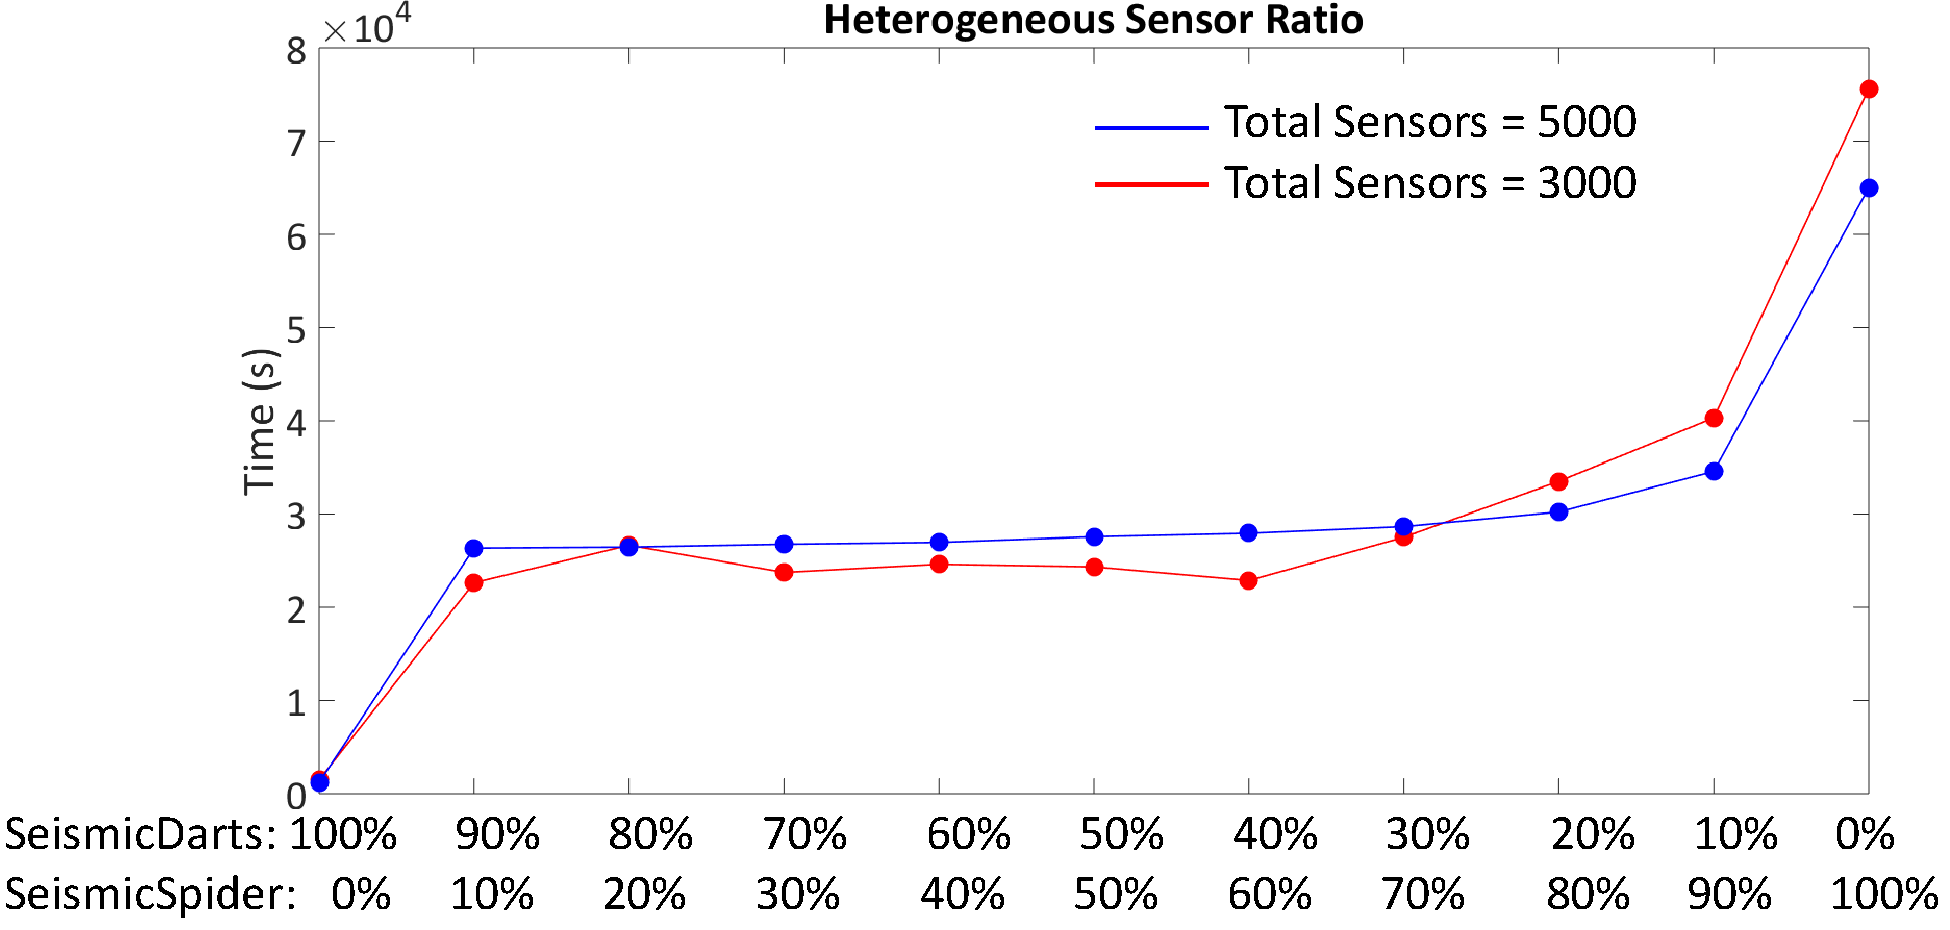
\includegraphics[width=\columnwidth]{ral2016/het_sen_ratio.pdf}}
 \caption{Survey time for different sensor ratios. The total number of sensors \{5000, 3000\} were kept constant. Ten darts were provided for each UAV. } 
 \label{fig:het_sen_ratio}
  \vspace{-1em}
\end{figure}

\subsection{Simulation Studies}
   A scheduling system to compare  time and costs for seismic surveys with varying numbers of UAVs, SeismicSpiders, SeismicDarts, and human laborers was coded in  {\sc Matlab}, available at \cite{Srikanth2016seismicScheduler}.
% The goal of the Seismic Survey Scheduler is to estimate the requirements for a specific seismic survey. 
% The scheduler compare  time and costs for seismic surveys with varying numbers of UAVs, SeismicSpiders, SeismicDarts, and human laborers was coded in  {\sc Matlab}, available at \cite{Srikanth2016seismicScheduler}. 
   In each simulation, a seismic source must be measured at every survey point. 
   The scheduler must assign each sensor (SeismicDart or SeismicSpider) to an unmeasured survey point and assign each UAV or human worker a dart to pickup or deploy.  Once a sensor reaches a survey point, that sensor must wait until a seismic source is measured.
   A vibration truck (blue) provides the seismic source.
   Motion planning uses a centralized, greedy strategy.
   
   Frames from four different cases on a small survey region are shown in Fig.~\ref{fig:Sim_overview} on a 100x100 m area with survey points at 10 m spacing:
   a.) simulates 10 SeismicSpiders;  
   b.) simulates 5 SeismicUAVs deploying 50 SeismicDarts. Each UAV was allowed to carry up to 4 darts;
   c.) simulates 10 SeismicSpider, 5 SeismicUAVs and 50 SeismicDarts;
   d.) simulates 5 human workers deploying 75 SeismicDarts. Each worker was allowed to carry up to 10 darts. 
 Survey points are grey circles if unmeasured and green if measured.   The simulation uses red hexagons for SeismicSpiders,  black diamonds for UAVs,  inverted yellow triangles for SeismicDarts, and magenta diamonds for human workers. The assigned motion path for each sensor is colored magenta and the path completed is blue. 
 %The program simulates a seismic survey and records the time required. This allows comparing different combinations of sensing assets.

   
%  The first frame in Fig.~\ref{fig:Sim_overview} corresponds to SeismicSpiders (red hexagons) surveying a area of 100x100 m. 
%  Ten SeismicSpiders moving at a velocity of $0.1$m/s tries to visit each survey point (indicated by blue circles) on the map. 
%  Once ten of these sensors are at a new survey location the blue truck (Seismic source) perturbs the ground creating a seismic wave. The SeismicSpiders record the values at their current locations. 
%  Then they start moving to their next location and we repeat this process until we obtain readings at the survey locations. 
% % We follow a greedy approach to identify the SeismicSpiders new location.
%   The second frame in Fig.~\ref{fig:Sim_overview} corresponds to SeismicUAV (Black Diamond) deploying the SeismicDarts (inverted yellow triangle).
%    One SeismicUAV can carry four SeismicDarts simultaneously and drop them at different locations. 
%    Similar to the simulation involving the SeismicSpider once ten sensors are at a new survey point the blue truck takes a shot. 
%    The SeismicDarts record the readings at their corresponding locations.
%     Once this is done the SeismicUAV will pick up these SeismicDarts and redeploy them at new survey point.
%     % We follow a greedy approach to deploy these sensors. 
%      The third frame in Fig.~\ref{fig:Sim_overview} combines the SeismicSpider and SeismicDarts.
%       This represents a heterogeneous system surveying. 
%       The fourth frame in Fig.~\ref{fig:Sim_overview} represents human workers (magenta diamonds) servicing a region.
%        In all the simulations red lines connect the sensor location the sensor just surveyed to it's new location. 
%        The blue line connects the location the sensor just surveyed to it's current location. 
%        All sensors are assumed to start from the blue truck at $T = 0$. 
%        The Seismic Survey  simulates the proposed system and comparison with manual deployment could be achieved for analysis. 
%        The simulator is robust and all the parameters described above are variables. 
%        We want this tool to be used for preprocessing of a seismic survey in which you can vary the number of sensors, velocity, size of seismic survey, location of the seismic source etc.
%         Using this simulator we can closely match a real seismic survey and thus optimize the resources.
 

%A scheduling system to compare  time and costs for seismic surveys with varying numbers of UAVs, SeismicSpiders, SeismicDarts, and human laborers was coded in  {\sc Matlab}, available at \cite{Srikanth2016seismicScheduler}. Frames from four different cases are shown in Fig.~\ref{fig:Sim_overview}.

This tool allows us to examine engineering and logistic trade-offs quickly through simulations.  For example, Fig.~\ref{fig:DronevsTime} assumes a fixed number of darts and examines the finishing time with $5$ to $500$ UAVs.  The time required decays asymptotically, but $140$ UAVs requires only twice the amount of time required for $500$ UAVs, indicating  $140$ UAVs are sufficient for the task.    
 Substantial cost savings can be obtained by selecting the number of UAVs required to complete within a certain percentage greater than the optimal time.

The tool is useful for comparing the effectiveness of heterogeneous teams.  Table~\ref{tab:Sim_table} compares surveying a $1$ km x $10$ km strip of land with teams of (a) $5000$ SeismicSpiders, (b) $500$ UAVs and $5000$ SeismicDarts, (c) $500$ humans and $5000$ geophones.  Team (b) completed six times faster than team (c). 
  Since SeismicSpiders are  slower than UAVs and humans and are expensive compared to the SeismicDarts, their use is limited to special occasions. The UAV can deploy the SeismicSpider at a given waypoint. This attribute was not considered in the simulation but would improve deployment speed of SeismicSpiders.
   
In Fig.~\ref{fig:het_sen_ratio}, the total number of mobile agents are constant, but the percentage of UAVs and SeismicSpiders are varied.  10 SeismicDarts were provided for each UAV. Increasing the percentage of UAVs lowers the deployment time because UAVs move 20 m/s but SeismicSpiders move 0.2 m/s. 
The velocity difference makes UAV deployment time-efficient. 
